\documentclass[tikz,border=5mm]{standalone}
\usepackage{tikz}
\usetikzlibrary{arrows.meta, positioning, shapes.geometric, calc, patterns}

% --- COLOR DEFINITIONS ---
\definecolor{Garnet}{HTML}{73000A}
\definecolor{CBlue}{HTML}{466A9F}
\definecolor{CDark}{HTML}{1F414D}
\definecolor{CGold}{HTML}{A49137}
\definecolor{CGrayLight}{HTML}{E5E5E5}
\definecolor{CGrayDark}{HTML}{555555}
\definecolor{CWhite}{HTML}{FFFFFF}

\begin{document}

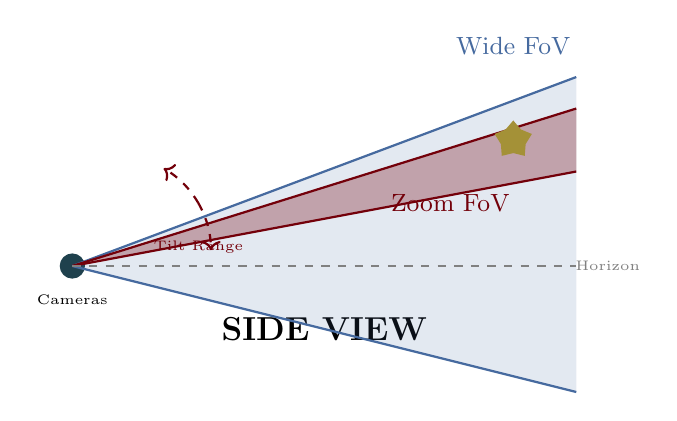
\begin{tikzpicture}[scale=0.8]
    % Title
    \node[font=\bfseries\large] at (4, -1) {SIDE VIEW};
    
    % Cameras (appear as one dot since they are side-by-side in this view)
    \fill[CDark] (0, 0) circle (0.2);
    \node[below, font=\tiny] at (0, -0.3) {Cameras};
    
    % Wide FOV (Blue) - Vertical spread
    \fill[CBlue, opacity=0.15] (0, 0) -- (8, 3) -- (8, -2) -- cycle;
    \draw[CBlue, thick] (0, 0) -- (8, 3);
    \draw[CBlue, thick] (0, 0) -- (8, -2);
    \node[CBlue, font=\small] at (7, 3.5) {Wide FoV};
    
    % Zoom FOV (Red) - Narrow, tilted upward to track target
    \fill[Garnet, opacity=0.3] (0, 0) -- (8, 2.5) -- (8, 1.5) -- cycle;
    \draw[Garnet, thick] (0, 0) -- (8, 2.5);
    \draw[Garnet, thick] (0, 0) -- (8, 1.5);
    \node[Garnet, font=\small] at (6, 1) {Zoom FoV};
    
    % Target
    \node[star, star points=5, fill=CGold, minimum size=0.4cm] at (7, 2) {};
    
    % Tilt arrows
    \draw[->, Garnet, dashed, thick] (2, 1) arc (30:60:1.5);
    \draw[->, Garnet, dashed, thick] (2, 1) arc (30:0:1.5);
    \node[Garnet, font=\tiny] at (2, 0.3) {Tilt Range};
    
    % Horizon line
    \draw[gray, dashed] (0, 0) -- (8, 0);
    \node[gray, font=\tiny] at (8.5, 0) {Horizon};
    
\end{tikzpicture}

\end{document}
